
%(BEGIN_QUESTION)
% Copyright 2014, Tony R. Kuphaldt, released under the Creative Commons Attribution License (v 1.0)
% This means you may do almost anything with this work of mine, so long as you give me proper credit

Suppose you needed to measure the voltage output by a combination pH electrode immersed in a liquid solution, but the only instruments you possessed to make this measurement were a set of standard digital multimeters (DMMs).  You happen to know that the ``null-balance'' or ``potentiometric'' method of voltage measurement will allow you to measure the pH probe's output signal even with low-impedance meters.  Sketch a diagram for a ``null-balance'' voltage measurement circuit connected to the pH probe.  Feel free to add other passive (non-amplifying) electronic components as needed to make your test circuit complete:

$$\includegraphics[width=15.5cm]{i00965x01.eps}$$

Also, explain why the ``null-balance'' technique works to measure the output voltage of a pH probe, whereas a direct-connected DMM will give false readings.

\underbar{file i00965}
%(END_QUESTION)





%(BEGIN_ANSWER)

5 points for proper sketch (all or nothing), 5 points for correct explanation:

\vskip 10pt

Multiple solutions exist (including using a variable DC power supply rather than a battery and potentiometer), but in any case the solution must have the voltmeter connected in parallel with an adjustable DC voltage, and an ammeter connected in series with the pH probe to indicate zero current.
 
$$\includegraphics[width=15.5cm]{i00965x02.eps}$$

\vskip 10pt

The ``null-balance'' technique ensures no current is drawn from the voltage source under test, in this case the pH probe.  If there is no current drawn from the source, its source impedance becomes irrelevent.  A direct-connected DMM will give falsely low readings due to its loading effect on a high-impedance voltage source.

%(END_ANSWER)





%(BEGIN_NOTES)

{\bf This question is intended for exams only and not worksheets!}.

%(END_NOTES)


